\section{introduction}
More than half a century after their discovery, quasars still maintain the interest of a productive part of the astrophysical community. Although several mechanisms have been proposed 
to explain how such systems function, a single mechanism is widely accepted at the present time. The model was first proposed by \cite{1964ApJ...140..796S}, followed by \cite{1964SPhD....9..246Z} in the same year and \cite{1969Natur.223..690L} five years later. The present name of the model is the Super-Massive Black Hole (SMBH) paradigm.\\

According to the paradigm, the object is powered through the accretion of matter from the proximal environment into the black hole. The radiation emitted excites the surrounding medium which becomes detectable as the narrow line regions,
broad band regions and torus. Moreover, in the direction perpendicular to the accretion disk, where the medium is more transparent, jets will appear. When the medium between and observer and such an object is transparent a quasar can be observed (citation). In other words an active galactic nucleus (AGN) with one of the poles orientated towards Earth would be detected as a quasar by an observer. \\

Through extensive observations done in the past 50 years, an important part of the assumptions and details  regarding the mechanism have been confirmed and uncovered. Still, the black hole shadow and the surrounding luminous accreting material (the black hole silouette) remains to be probed. Advancements in the very long baseline interferometer observations have made possible since 2007, the detection of structures of a few Schwarzschild radii at the Sagitarius A object at the center of our galaxy \citep{2008JPhCS.131a2055D}. Furthermore, jet launching structure near the supermasve black hole in M87 were resolved with the same observation tool \citep{2012Sci...338..355D}. With all the advancement, the current number of baselines does not allow the direct generation of images from the observations still it does allow the fitting of the data to predefined models \citep{2013MNRAS.434..765K}.


A whole range of models have been applied starting from simple geometric models to more complex, physically sensible models (Doeleman et al 2008, Fish et al 2011, Broderick et al 2011, Moscibrodzka et al 2009, Dexter 2010 and others). A significant fraction of the later models predict a crescent shaped silouette of the black hole. This motivated \cite{2013MNRAS.434..765K} to use a simple geometric crescent model to fit the data. The succesfull results encouraged the authors to speculate that the shadow of the black hole will be observed in the near fututre with the previously mentioned observation method. \\


Hundreds of thousands of quasars have been detected up to date, mainly from the Sloan Digital Sky Survey. The great majority of them present a redshift larger than 2.15 of their spectra (Paris et al 20Nov 2013 SDSS catalogue). Therefore the typical distance to the objects is in the order of gigaparsecs  or above. A value that is orders of magnitude larger than the distance to M87. Direct observation of the black hole silouette of quasars require significant technological advances. We argue in the present paper
 that one can probe and study the black hole shadow and its proximal environment belonging to a quasar without having to resolve sub-event horizon scales. We consider that this is possible by analyzing the data from microlensing-events.  Moreover, unlike with the few nearby AGNs, the study of the very large quasar population allows for the statistical refinement of the global properties of AGN by highlighting any particular
characteristic that is present only in SGA* and M87 central region. Furthermore, by probing the event-horizon-scale inner regions of a large number of objects will facilitate the study of the evolution of the previously mentioned region.     
     
Gravitational microlensing of QSOs have been predicted as early as 1981 when \cite{1981ApJ...243..140G} suggested that ''if haloes of galaxies were composed of stars with masses less than  0.1 $M_{sol}$, then these stars acting as individual lenses whould produce fluctuations of the order of 
unity in the intensities of the QSO images on time scales of 1 -14 years '' (Gott 1981). What creates the magnification event is the relative and independent motion of the lens and source with respect to the observer. Since the respective lens is surrounded by similar objects one would expect to observe during a long enough time interval
multiple microlensing events of the same source, the QSO. The sequential alignment of the source and observer with different lensing objects will result in an aparently random increase of the QSO light flux analogous to the scintilation events in a meter of radioactivity.

Estimates of the Einstein radius for the particular case of a QSO at redshift 2 lensed by a compact stellar mass object at redshift 0.5 was found to be $10^-6 \sqrt{M/M_{sol}} arcsec$ \citep{2001PASA...18..207W}. The Schwarzschild radius of the Sgr A* black hole, situated at 8 kpc from Earth \citep{1993ARA&A..31..345R} spans an angle of 10 microarcsec on the sky \citep{2008JPhCS.131a2055D}. If the quasars observed at z =2 would have similar linear sizes, the aparent size of the  luminous part of the QSO would be many orders of magnitude below the 1 microarcsec level. Therefore the aparent size would be significantly smaller than the corresponding Einstein radius of a solar mass lens. 
The magnitude differences between the Einstein angle and the aparrent size of the bright part of the QSO motivates the introduction in the first part of the paper of simplified models for     
calculating the lightcurves of QSO magnification events. The simplified models are introduced in the theory section of the present paper. In the theory (II) section of the present article with an introduction to the basic microlensing theory in which we present the general microlensing equation followed by the concept of magnification. We underline that for the particular case of micro gravitational lensing,
the images are not resolved and thus the magnifications of each images contribute to a total magnification. Furthermore, the concept of critical curves and caustics are introduced. Afterwards we focus on a particular singularity, namely the fold singularity. We choose to study events related to the previously mentioned singularity since the magnification events caused by the crossing of such boundaries are most probable. A quick inspection of figure 1 by the reader should motivate the previous statement. 
In continuation we introduce the commonly used result involving the magnification of a point-like source near a fold singularity. Namely that the magnification is aproximately linear outside the caustic and decreases from infinity with the square root of the distance to the boundary when inside the caustic.  
In the last section of the Introduction (II) we present the general equations for estimating the flux received from an extended source near a fold. The only elements required to compute the flux as a function of time are the two dimensional brightness function of the object and the magnification of a point-like source. One of the core
assumptions made when developing the simple models is that the einstein angle is orders of magnitude greater than the apparent size of the source. Due to this assumption one can imagine the caustic as an infinite wall to be crossed by the source as presented in figure 2. The consequence of the limit is that the information regarding the profiles of the source along any direction parallel to the boundary value is reduced to the corresponding integral value. The effect allows the introduction of a one dimensional flux function, which is the two dimensional flux integrated along the axis paralel to the boundary. The one dimensional profile contains exhaustively all the information that can be extracted  from the lens generated light-curve \\

\begin{figure}
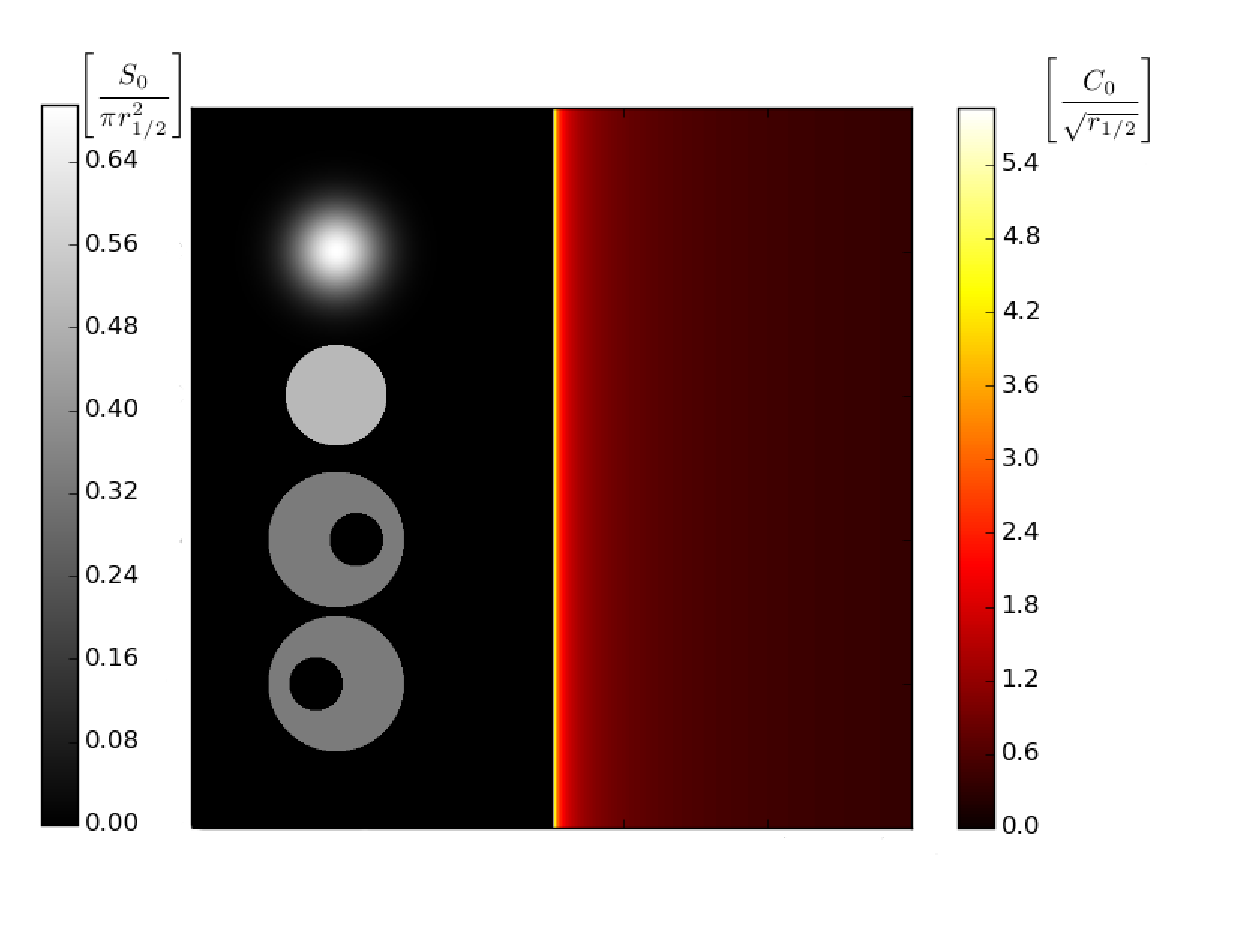
\includegraphics[width = .8\textwidth]{plots/infinite_fold.eps}
\caption{\label{fig:infinite_fold}  Source profiles and magnification map for an infinite fold. Objects have the same $S_{0}$ and $r_{1/2}$ }
\end{figure}




In the third section we introduce the three source profiles used in our models and simulations. We start with two commonly used and simple sources. Namely the gaussian brightness distribution and the constant intensity disk. In addition we use a geometric crescent-shaped source effectively the same as the one introduced by \citep{2013MNRAS.434..765K} with constant surface brightness. \\
The fourth section contains the results of our simplified models calculations, including the numerical equation for lightcurve calculations and the corresponding plots. In order to facilitate comparison bewteen the lightcurves of the three distinct sources, we constrain the luminosity and half-light radius of all sources to have the same value.    
       
We continue to the second part of the paper, where we have advanced the level of complexity of our models. Using the Wambsganss gravitational lensing code (citation) a realistic magnification map is generated. The magnification map replaces the simplified magnification function used previously.  \\
The numerical method, hierachical tree structure and backwards reatracing, underlying the microlensing code is treated in section five. Aside from a basic review of the physical and numerical principles of the code, the description of its generalization from disk shaped source images to crescent ones can be found here as well. Further, the mass distribution in the lens plane, chosen to produce the magnification map used in this analysis, is introduced and motivated.   
